\section{Auswertung}

\subsection{Direkte Messung der Leerlaufspannung}

Der Eingangswiderstand des Voltmeters beträgt
\begin{equation*}
  R_V = \SI{10}{\mega \ohm} = \SI{1e7}{\ohm}.
\end{equation*}

Die direkte Messung ergibt für die Leerlaufspannung
\begin{equation*}
  U_0 = \SI{1,4}{\V}.
\end{equation*}

\subsection{Messung des Innenwiderstandes einer Monozelle \label{sec:uk}}

Die aufgenommenen Messwerte befinden sich in Tabelle \ref{tab:uk}.
\begin{table}[H]
  \centering
  \caption{Messdaten für die Klemmenspannung}
  \label{tab:uk}
  \begin{tabular}{S S}
    \toprule
      {$I \:/\: \mathrm{mA}$} & {$U_k \:/\: \mathrm{V}$}\\
    \midrule
    22,0  &  1,20  \\
    22,0  &  1,20  \\
    23,5  &  1,20  \\
    27,5  &  1,15  \\
    29,5  &  1,15  \\
    33,0  &  1,15  \\
    39,0  &  1,10  \\
    47,0  &  1,05  \\
    59,0  &  1,00  \\
    73,0  &  0,90  \\
    98,0  &  0,70  \\
    190,0  & 	0,05 \\
    \bottomrule
  \end{tabular}
\end{table}

Aus diesen Messwerten folgt Graph \ref{fig:uk}:
\begin{figure}[H]
  \centering
  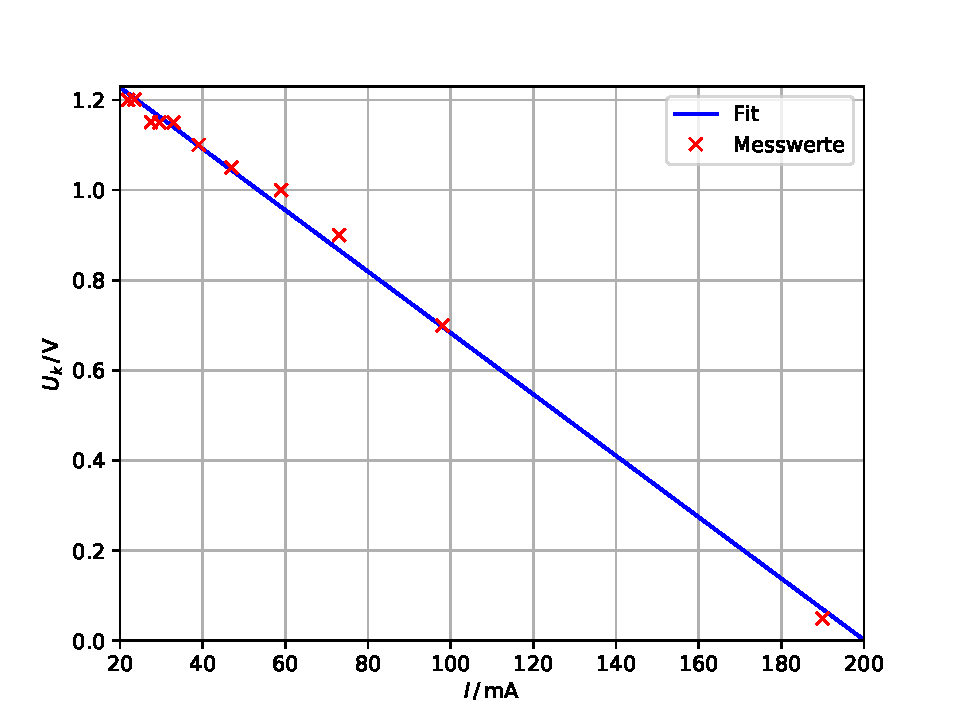
\includegraphics[width=\textwidth]{Plots/uk.pdf}
  \caption{$U_k$-$I$-Diagramm zur Bestimmung des Innenwiderstandes}
  \label{fig:uk}
\end{figure}

Mithilfe der Messwerte wird die lineare Regression $- a \cdot x + b$ durchgeführt, die die Werte
\begin{align*}
  a &= \SI{6,810(131)}{\ohm} \\
  b &= \SI{1,364(9)}{\V}
\end{align*}

liefert. Dabei ist $a$ der Innenwiderstand $R_i$ und $b$ die Leerlaufspannung $U_0$.

% Die Fehler erhält man aus der Gauß'schen Fehlerfortpflanzung
% \begin{equation}
%    \delta = \sqrt{ \sum_{i=1}^{n}(\frac{\partial y}{\partial x_i} \Delta x_i)^2}.
%    \label{eqn:gaus}
%  \end{equation}


\subsection{Messung mit einer Gegenspannung \label{sec:ukmg}}

Die aufgenommenen Messwerte befinden sich in Tabelle \ref{tab:ukmg}.
\begin{table}[H]
  \centering
  \caption{Messdaten für die Klemmenspannung}
  \label{tab:ukmg}
  \begin{tabular}{c S}
    \toprule
      {$I \:/\: \mathrm{mA}$} & {$U_k \:/\: \mathrm{V}$} \\
    \midrule
    22  &  2,10  \\
    33  &  2,05  \\
    40  &  2,00  \\
    44  &  2,00  \\
    51  &  1,95  \\
    58  &  1,90  \\
    74  &  1,80  \\
    83  &  1,75  \\
    \bottomrule
  \end{tabular}
\end{table}

Aus diesen Messwerten folgt Graph \ref{fig:ukmg}:
\begin{figure}[H]
  \centering
  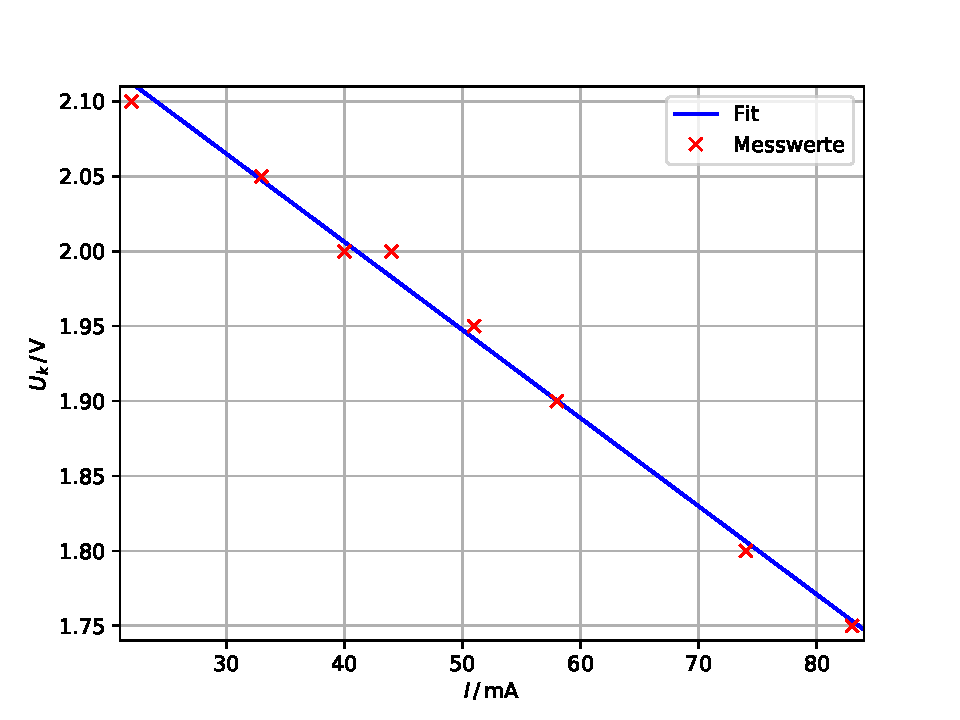
\includegraphics[width=\textwidth]{Plots/ukmg.pdf}
  \caption{$U$-$I$-Diagramm zur Bestimmung des Innenwiderstandes}
  \label{fig:ukmg}
\end{figure}

Es wird erneut eine lineare Regression durchgeführt. Sie liefert die Werte
\begin{align*}
  a &= \SI{5,882(187)}{\ohm} \\
  b &= \SI{2,242(10)}{\V}
\end{align*}

\subsection{Messung des Innenwiderstandes eines Rechteckgenerators}

Die aufgenommenen Messwerte befinden sich in Tabelle \ref{tab:rechtuk}.
\begin{table}[H]
  \centering
  \caption{Messdaten für die Klemmenspannung}
  \label{tab:rechtuk}
  \begin{tabular}{S S}
    \toprule
      {$I \:/\: \mathrm{mA}$} & {$U_k \:/\: \mathrm{V}$} \\
    \midrule
    2,8  &  0,55  \\
    3,0  &  0,54  \\
    3,3  &  0,53  \\
    3,7  &  0,51  \\
    4,2  &  0,49  \\
    4,8  &  0,46  \\
    5,6  &  0,43  \\
    6,1  &  0,40  \\
    7,6  &  0,34  \\
    8,1  &  0,24  \\
    15,0  &  0,16  \\
    \bottomrule
  \end{tabular}
\end{table}

Aus diesen Messwerten folgt Graph \ref{fig:rechtuk}:
\begin{figure}[H]
  \centering
  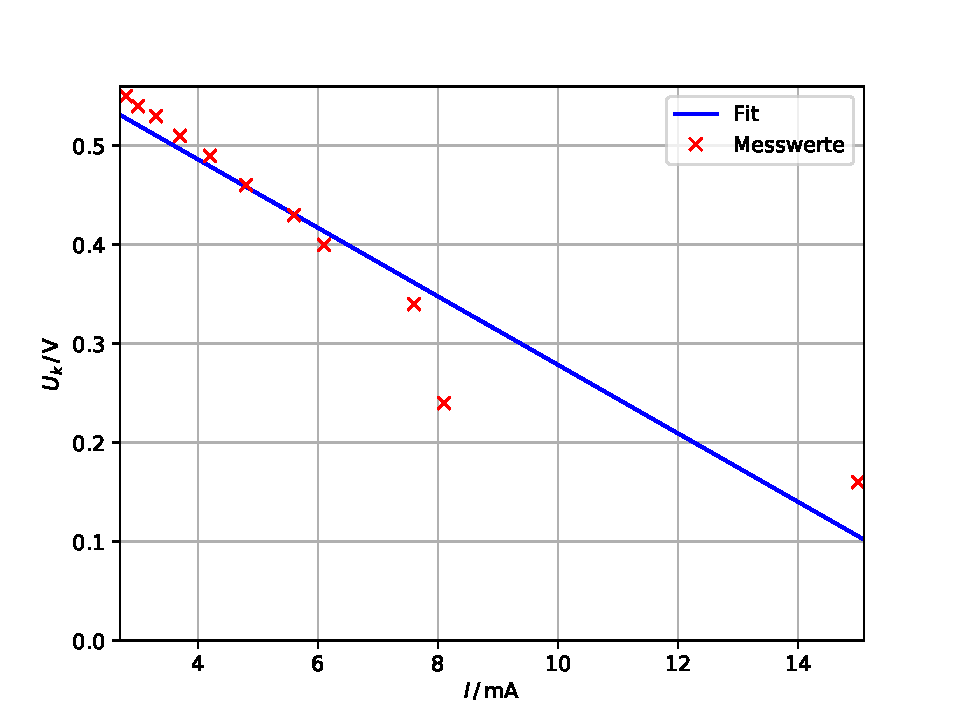
\includegraphics[width=\textwidth]{Plots/rechtuk.pdf}
  \caption{$U$-$I$-Diagramm zur Bestimmung des Innenwiderstandes}
  \label{fig:rechtuk}
\end{figure}

Dieses mal ergibt die lineare Regression
\begin{align*}
  a &= \SI{34,590(3786)}{\ohm} \\
  b &= \SI{0,625(26)}{\V}.
\end{align*}

\subsection{Messung des Innenwiderstandes eines Sinusgenerators}

Die aufgenommenen Messwerte befinden sich in Tabelle \ref{tab:sinuk}.
\begin{table}[H]
  \centering
  \caption{Messdaten für die Klemmenspannung}
  \label{tab:sinuk}
  \begin{tabular}{S S}
    \toprule
      {$I \:/\: \mathrm{mA}$} & {$U_k \:/\: \mathrm{V}$} \\
    \midrule
    0,15  &  1,95  \\
    0,20  &  1,95  \\
    0,25  &  1,90  \\
    0,30  &  1,90  \\
    0,35  &  1,85  \\
    0,40  &  1,80  \\
    0,55  &  1,75  \\
    0,75  &  1,60  \\
    1,10  &  1,40  \\
    1,65  &  1,05  \\
    2,40  &  0,60  \\
    \bottomrule
  \end{tabular}
\end{table}

Aus diesen Messwerten folgt Graph \ref{fig:sinuk}:
\begin{figure}[H]
  \centering
  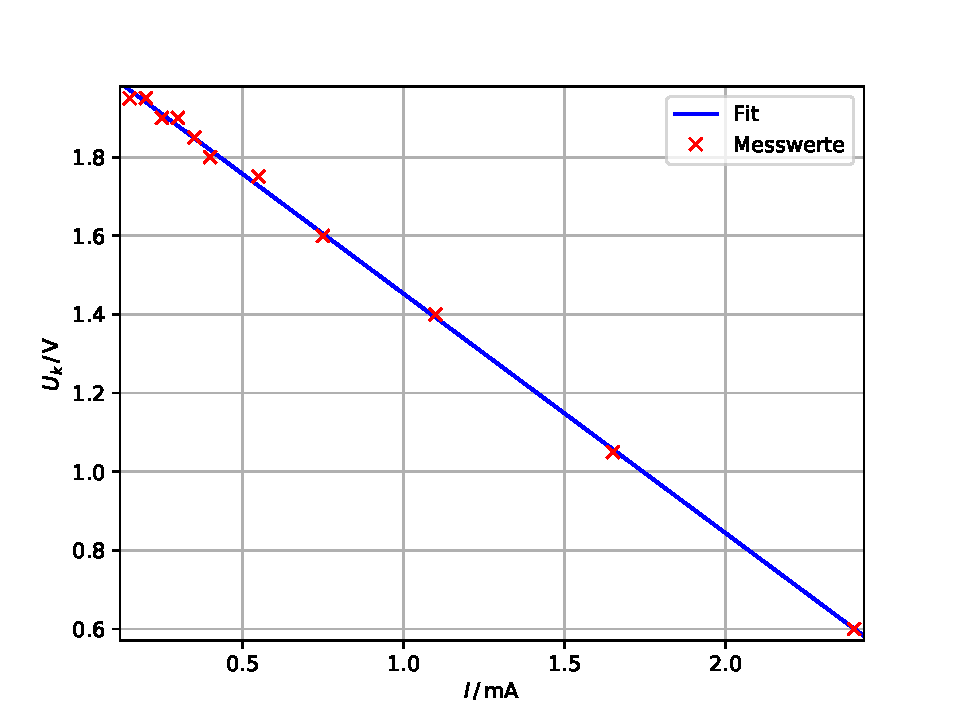
\includegraphics[width=\textwidth]{Plots/sinuk.pdf}
  \caption{$U$-$I$-Diagramm zur Bestimmung des Innenwiderstandes}
  \label{fig:sinuk}
\end{figure}

Die lineare Regression ergibt
\begin{align*}
  a &= \SI{609,072(6695)}{\ohm} \\
  b &= \SI{2,062(7)}{\V}.
\end{align*}

\subsection{Systematische Fehler \label{sec:sysf}}

Da das Voltmeter nur einen endlichen Widerstand hat, ergibt sich ein systematischer Fehler
bei der direkten Messung der Leerlaufspannung.
Der Fehler ergibt sich als
\begin{equation*}
  \delta = \frac{R_i}{R_a} = 6,81 \cdot 10^{-5} \%.
\end{equation*}

Da der Fehler so klein ist, wird er vernachlässigt.
Das Voltmeter an den Punkt H anzuschließen würde einen weiteren systematischen Fehler versursachen.
Es wäre nicht mehr möglich die reine Klemmenspannung zu messen, weil die über dem nicht idealen Amperemeter
abfallende Spannung mitbetrachtet werden würde.

\subsection{Leistung}

In Graph \ref{fig:leistung} wird die Leistung gegen den Lastwiderstand aufgetragen.
Diese Größen berechnen sich aus
\begin{align}
  P &= U_k \cdot I & R_a &= \frac{U_k}{I}
\end{align}
\begin{figure}[H]
  \centering
  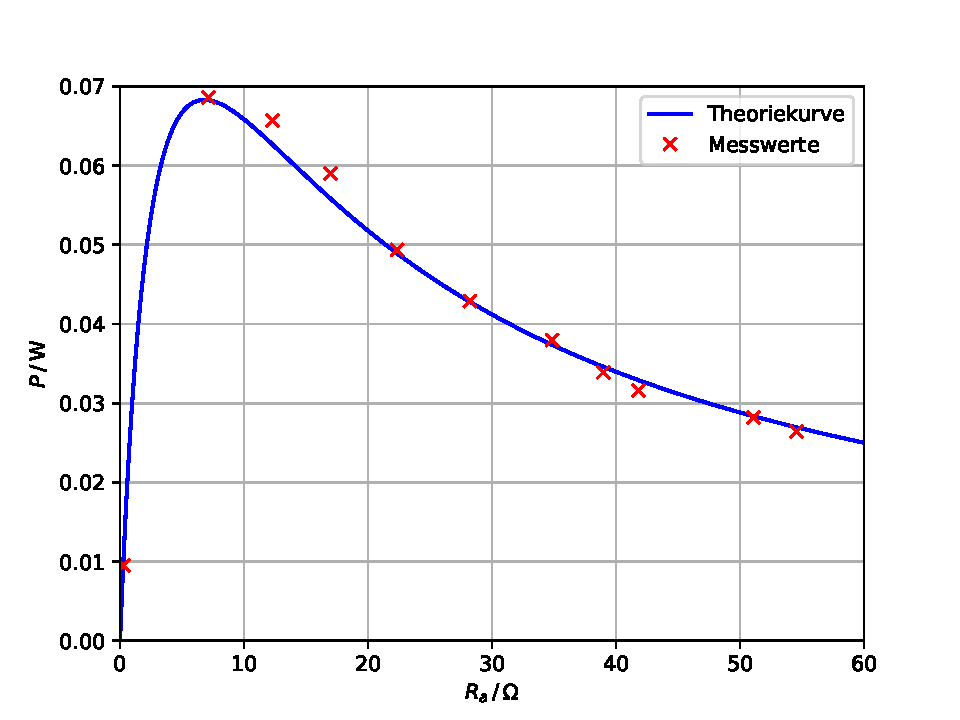
\includegraphics[width=\textwidth]{Plots/leistung.pdf}
  \caption{$P$-$R_a$-Diagramm}
  \label{fig:leistung}
\end{figure}

Die Theoriekurve ergibt sich aus Gleichung \eqref{eqn:leistung}.
